\section{Efficient Feature Maintenance}

In this section, we formalize the feature maintenance problem addressed in this paper, that is, selecting the keys for \cref{lst:cache-maintenance}. 
In a resource-constrained setting, only a subset of features can be updated at any given time, resulting in feature staleness which may degrade prediction accuracy. The focus of this paper is precisely to optimize this issue: deciding which keys to update in response to new data, with the objective of maximizing downstream prediction accuracy. As previously highlighted, the core enabling factor is the differentiated impact that feature staleness has on overall accuracy: stale features may lead to low query errors, while some features may simply rarely be queried at all. \amit{different features will have different impacts on downstream accuracy, as some features might rarely be queried whereas others might contribute significantly to the model's output.}
\jmh{Next sentence needs grammar fix, and should be an echo of the intro! If you find yourself typing "this is the focus of the paper" in Section 3 it means you're concerned that Section 1 failed to do its job. "\emph{The focus of this paper is precisely to optimize this issue: deciding which keys to update in response to new data, with the objective of maximizing downstream prediction accuracy.}"}

\natacha{This paragraph felt a little strange as you've already said this multiple times in S1 and S2, but you've written it in a way that makes it sounds like it's new information. I added three lines and vote to remote the rest of this paragraph. TEMPORARILY COMMENTED OUT}
%The impact of feature updates on accuracy can vary with the query distribution over features and the the impact of the new data on the current feature value. In some cases, the frequency of data changes may be uncorrelated with the query pattern from downstream applications, resulting in frequent updates to keys that are seldom queried, as show in \cref{f:updates_vs_queries}. Even for features queried with similar patterns, the importance of incoming data updates may vary. Some updates may radically change predictions; others may have little impact on predictions and can be deferred or ignored. 
%For example, the first few comments on an article can have a significant impact on the rating of that article. In contrast, later comments may have a negligible impact in downstream prediction accuracy. Similarly, largely redundant or uninformative comments on an article are unlikely to affect user preferences.
%


%At the same time, there is more flexibility \jmh{more than what?} with how features are maintained \natacha{Compared to what?}. In contrast to traditional caches that must fully invalidate entries with changes in the data, stale features have the \emph{potential} of negatively impacting accuracy.  \natacha{For what it's worth, I never really thought of features as caching, more thought of them as a materialization, so this sentence didn't resonate with me a lot}






% Furthermore, we have a clearly defined objective of minimizing the impact of inaccurate features on the downstream prediction accuracy. 
% \natacha{The last three sentences seem strewn together but don't seem to follow logically from one another}


\natacha{It would be cool to have a separate section that makes a bigger deal out of this, right now it's a little lost in everything else. We know how hard staleness and weak consistency is to deal with, but now we have a solution! We can actually numerically assess what the true cost of weak consistency. It's huge!}



\subsection{Feature Approximation} 
\label{sec:approximation}
%The cost of feature maintenance can be reduced by introducing approximation to the way the feature values are maintained. 


%Calculating $v^t_k$ at each timestep for all keys is often prohibitively expensive, necessitating that feature values are approximated with some $\tilde{v}_k^t$. We can approximate $\tilde{v}_k^t$ by approximating the featurization (e.g. with data sub-sampling \cite{wedge2018solving} or using a lighter-weight feature function \cite{willump}), or by using past (stale) version of the feature value. In this work, we focus on the latter mechanism by choosing what keys to update and what keys to keep the stale values for. 

%\subsubsection{Stale Features} 
Featurization cost can be reduced by computing features using approximated featurization (e.g. sampling) or using stale features, which is the focus of this paper. Reducing the frequency of updating feature values by tolerating staleness is a simple way to reduce featurization cost, as the same update function can be used on the same data: the only parameter to change is when the update is triggered. For example, multiple edits to a document can be batched together so the document only needs to be re-embedded once, or a function over a window of data can be run less frequently to reduce computational cost. 


For feature derived from data $\mathcal{D}^{t}$, we denote the true feature values at time $t$ as $v^t_k = f\left( \mathcal{D}^{t}_k\right)$, and the stale feature values as 
\begin{equation}
    \tilde{v}^t_k = f\left( \mathcal{D}^{t-\delta_{k,t}}_k\right).\label{eqn:delayedupdate}
\end{equation}
% We formally denote the approximation achieved by delaying updates as: 
% \begin{equation}
%     \tilde{v}^t_k = f\left( \mathcal{D}^{t-\delta_{k,t}}_k\right).\label{eqn:delayedupdate}
% \end{equation}
where $\delta_{k,t}$ is the staleness of the current feature value.  Delaying update processing, and thereby increasing the staleness, reduces how often $f$ needs to be run on new data. However, reducing the frequency of re-computation results in features that are more stale, as entries in the feature table are more likely to be missing the most recent updates. 

\subsubsection{Evaluating Approximation Quality} Standard ways to evaluate the quality of approximation is to evaluate the staleness of the queried data, or the differences in the approximated and unapproximated value. However in the context of feature stores, these metrics do not necessarily correlate to prediction quality. Feature staleness or large divergence in feature values is not problematic if the prediction quality is not impacted. Similarly, slight changes in the feature values can dramatically change predictions\sarah{try to cite something}. For example, neural networks can be very sensitive to small perturbations in input, and it is difficult to model how differences in feature values will correlate to differences in predictions, especially when the input values to the model are unknown.  \sarah{try to cite something}

However, directly using downstream accuracy as a metric for feature quality is problematic, as prediction quality depends on \textit{both} the features and the model. A model may perform poorly for an out-of-distribution user regardless of feature approximation quality. In order to disentangle model performance from feature quality, we propose \textit{feature store regret} in the next section. 

%We can denote approximate feature updates as:
%\begin{equation}
%    \tilde{v}^t_k =  f\left( s(\mathcal{D}^{t}_k)\right).\label{eqn:sampling}
%\end{equation}
%where $s$ is some sampling function that takes all the available data $\mathcal{D}^{t}_k$ at time $t$ and returns a subset of that data.
%Because feature computation often depends linearly or polynomially in the data size, sampling can significantly reduce computational costs often without significant impact on the feature store loss.



%In \cref{eqn:delayedupdate}, we delayed updates uniformly.  
%However, in practice we may choose to assign a separate delay $\delta_k$ for each key or even make the delay a lightweight function of $\delta(\mathcal{D}^t_k)$ of the data associated with that key.
%By prioritizing keys that are more likely to be accessed we can ensure that those keys will have more up-to-date features.
%In many settings, we would expect the query access pattern for features to be relatively stable providing strong signal for which keys are likely to be accessed in the future.

%Furthermore, not all data will result in significant changes to the feature values.  
%Therefore, we can prioritize updating features that have significant new data.


% \begin{figure}
% \centering
% \begin{subfigure}[b]{0.5\textwidth}
%    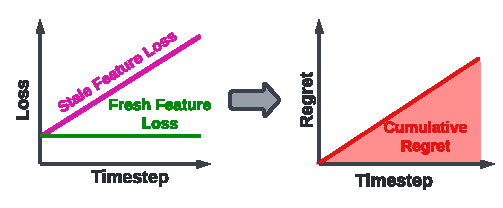
\includegraphics[width=8cm]{ralf/figures/regret_1.pdf}
%    \setlength{\abovecaptionskip}{-2pt}
%    \caption{Loss increases with staleness.}
%    \label{f:regret1} 
% \end{subfigure}

% \begin{subfigure}[b]{0.5\textwidth}
%    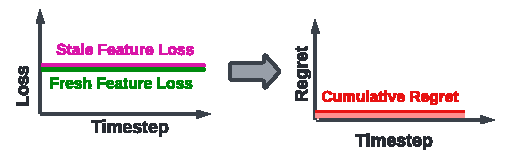
\includegraphics[width=8cm]{ralf/figures/regret_2.pdf}
%    \setlength{\abovecaptionskip}{-2pt}
%    \caption{Constant loss with staleness.}
%    \label{f:regret2}
% \end{subfigure}
% \setlength{\abovecaptionskip}{-0pt}
% \setlength{\belowcaptionskip}{-10pt}
% \caption{Examples of how the prediction loss of the ideal features (green) and the loss of the approximated/stale features (purple) might compare and corresponding regret. 
% %In (a.), increasingly staleness (assuming the feature was updated at t=0) degrades model prediction, and leads to rapidly increasing cumulative regret. In (b.) staleness does not affect the quality of the predictions. Regret still accumulates, but more slowly.
% }
% \label{f:cumulative-regret}
% \end{figure}

\subsection{Feature Store Regret}
\label{ss:regret}
% Approximating feature values to reduce compute resource costs poses the risk of degrading prediction quality of downstream models querying the features. We derive a metric to evaluate the approximation quality of features in terms of downstream prediction accuracy. 

% \subsubsection{Prediction Loss}
% We consider feature tables used in the context of online prediction serving, where models need to query feature values with low latency to process prediction requests. 
% Given a sequence of prediction request data $\{x_{kt}\}$ over keys $k$ and timestamps $t$, we can denote the sequence of predictions generated by the model $m$ in terms of current feature store values $v^t$:
% \begin{equation}
%     \hat{y}(v^t_k) = m\left(x_{kt}, v_k^t\right) 
% \end{equation}
% Each prediction corresponds to some $y$, the true label. The model is trained to minimize the loss $\ell(\hat{y}, y)$ (e.g. mean squared error or top-k error). We can formalize the prediction loss by the serving system as: 
% \begin{equation}
%     \mathcal{L}(m|v^t) = \mathbb{E}_{k\sim Q}\left[\ell\left(\hat{y}(v_t), y\right)\right]
% \end{equation}
% However, we cannot directly use loss to evaluate approximated feature values $\tilde{v}$. First, the true labels may not always be available, preventing observation of the loss. Second, the prediction loss if a function of both the feature values and the model parameters. If a model performs poorly for an out-of-distribution user, the feature store cannot correct the error by improving the quality of that user's features. However if the prediction quality is poor because of out-of-date features, the feature store should attempt to correct this.

%\subsubsection{Feature Store Regret}
We propose a feature store metric, \textit{feature store regret}, to evaluate feature quality. The feature store regret is the difference in predictions made by the optimal feature values $v_k^t$ and approximated features $\tilde{v}_k^t$. 
\begin{equation}
    \mathcal{R}(t) = \mathcal{L}(m|\tilde{v}^t) - \mathcal{L}(m|v^t)
\end{equation}
where $\mathcal{L}(m|\tilde{v}^t)$ and $\mathcal{L}(m|v^t)$ are the \textit{total loss} of predictions made with the approximated and unapproximated feature values, respectively. For simplicity, we assume $\mathcal{L}(m|\tilde{v}^t) \ge \mathcal{L}(m|v^t)$. We can write the total loss in terms of the sequence of prediction requests with data $\{x_i\}$ at time $t$ which correspond to predictions $\hat{y}_i(v_t)$ and true values $y_i$: 
\begin{equation}
     \mathcal{L}(m|v^t) = \sum_{i}\ell\left(\hat{y}_i(v_t), y_i\right)
\end{equation}
where $\ell$ is the loss function used to evaluate the model. 


\subsection{Scheduling with Error Feedback: Regret-Proportional Scheduling}
\label{ss:online-scheduling-error-feedback}
We propose an online scheduling policy in cases where we can observe regret online, which we refer to as \textit{Regret-Proportional} update scheduling. In many model serving applications, the true prediction label can eventually be observed. For example, a recommendation model can serve recommendations to a user and eventually observe which recommendations the user did or did not click through. Similarly, a time series \amit{model can have its predictions evaluated against future observed points}feature can be evaluated against future points observed for the time-series. The observations of the true label can be used to compute model prediction error, which can be used to provide feedback on feature quality. While prediction error cannot always be computed online, we constrain the problem to this setting to consider how error feedback can be used to make better scheduling decisions. 

We formalize the online scheduling problem for feature stores in terms of minimizing feature store regret under resource cost constraints.  At a high level, our proposed policy is to prioritize keys with the highest cumulative regret. 
%This allows us to prioritize updating keys where feature staleness has the highest impact on the overall loss (such as in \cref{f:regret1}) rather than keys where the prediction loss is primarily a result of model error (such as \cref{f:regret2}). 
This allows us to prioritize updating keys where feature staleness has the highest impact on the overall loss rather than keys where the prediction loss is primarily a result of model error. 
We describe how we estimate regret with error feedback in \cref{ss:scheduling-policy}. 
%Assuming the stale version of the feature is always available to be queried, we determine what keys to process updates for.

\subsubsection{Formulation}
We consider a feature table with keys $k\in K$ each mapping to values $\tilde{v}_k^t$. At time $t$, the scheduler can update a subset of keys $U_t \subseteq K$. For each $k\in U_t$, we recompute the feature value on all data up to the current timestamp, while other feature values remain the same. We can denote the approximate feature values at time $t$ with \cref{eqn:delayedupdate} where the staleness $\delta_{k,t}=0$ if the key $k$ is updated at time $t$, and otherwise $\delta_{k,t}=1+\delta_{k,t-1}$. 

Given a constraint $C$ on the number of keys which can be updated at each timestep $t$, our goal is to select updates $U$ such that the staleness matrix $\delta$ minimizes the cumulative regret over time: 
\begin{align}
     \argmin_\delta \sum_t \mathcal{R}(t) \\
     |U_t| \le C, \forall{t}
\end{align}
\subsubsection{Error Feedback}
We assume that we can observe the per-key loss. Say that for the sequence of queries $\{x_{kt}\}$, we eventually recieve error feedback $E_t = \{e_k\}$ denoting the prediction error of $m(x_{kt}, \tilde{v}_k^t)$. For simplicity, we assume that the error is received before we need to make scheduling decisions for the next timestep. We can estimate the per-key loss at each timestep as the sum $\mathcal{L}(m|\tilde{v}_t^ k) \approx \sum_{e_k \in E_t} e_k$.
\sarah{Maybe formalize t?}

\subsubsection{Scheduling Policy}
\label{ss:scheduling-policy}
We propose an online algorithm which selects keys to update based off the cumulative regret observed since the last update: 
\begin{equation}
   \argmax_k \sum_{s=0}^{\delta_{t,k}} \mathcal{R}_k(t-s) 
   \label{eq:cumulative_regret}
\end{equation}
\sarah{Define E TU}

%\subsubsection{Estimating Regret with Feedback}
To estimate $R(t)$, we also need an estimate of the loss with the ideal features $\mathcal{L}(m|v_t^ k)$. We assume that the \textit{expectation} of error over queries is temporally stable with respect to staleness for each key. Thus we can calculate the average error immediately after the feature was updated at time $t_u = t-\delta_{t,k}$ and multiply with the number of error observations at time $t$ to estimate $\mathcal{L}(m|v^t_k)$ and subtract this from each error value observed at timestamp $t$ before taking the sum of all errors observed at $t$. We can thus write out the estimated regret at $t$ as:
% , so we can approximate the unapproximated feature loss as a the loss observed right after the feature was updated (that is, at time $t-\delta_{t,k}$): 
% \begin{equation}
%     \mathcal{L}(m|v_t^ k) \approx |E_{t}|\cdot  \sum_{e_k \in E_{t-\delta_{t,k}}} \frac{e_k}{|E_{t-\delta_{t,k}}|} 
% \end{equation}
\begin{equation}
    \mathcal{R}_k(t) \approx \sum_{e_k \in E_{t}}  e_k -   \sum_{e_k \in E_{t_u}} \frac{ |E_{t}|\cdot e_k}{|E_{t_u}|}  
\end{equation}
Intuitively, we can think of this as computing how much additional error per query there is in $E_t$ (the current timestep error) as compared to $E_{t_u}$ (the post-update timestep error). Expanding out \cref{eq:cumulative_regret} and denoting the last update time as $t_u = t-\delta_{t,k}$, we select the key to update as:  
\begin{equation}
   \argmax_k \sum_{s=0}^{\delta_{t,k}} 
  \sum_{e_k \in E_{t-s}} \left( e_k -   \sum_{e_k \in E_{t_u}} \frac{ e_k}{|E_{t_u}|}  \right)
\end{equation}


%\subsubsection{No starvation} 
We can prevent starvation by upper bounding the regret $R_k(t) < \mathcal{R}_{max}$, and assuming $R_k(t) > \epsilon$ for some $\epsilon > 0$. We find in practice, since the errors in $E_{t_u}$ are relatively small, we can remove the second summation term and simply sum $e_k$ to estimate regret.

\subsubsection{Default Regret}
\label{ss:default-regret}
One potential issue with relying on cumulative regret for key prioritization is that a key may become arbitrarily stale if the key is never queried. Stale keys can be prioritized more by setting a higher minimum regret value $R_k(t) > \epsilon$, so that keys will incur regret over time.

